
\section{Voltage Transfer Curve}

\subsection{Procedure}

For the circuit shown in figure \ref{fig:circuit} we used the X-Y mode of our oscilloscope to find and display the voltage transfer curve. The value of the resistor was $R=295.3 \Omega$. Our power supply used an over-current protection of $200mA$, and a $V_{dd} = 10V$. The function generator used a sine wave with $V_{offset} = 5V$ and $V_{pp} = 10V$. Our output frequency was set to $f = 100 Hz$. This acted as $V_{in}$ on our reference circuit from figure \ref{fig:circuit}.

\FloatBarrier

\subsection{Results}
With the X-Axis corresponding to the $V_{in}$ and the Y-Axis corresponding to the $V_{out}$ we see the resulting VTC graph in figure \ref{fig:vtc_result}. From this graph we found that our threshold voltage is $V_{tn}\approx 2.0V$. This is consistent with the provided values in the manufacturer's data sheet that listed the threshold voltage as a range from $0.8 V \le V_{tn} \le 3.0 V$.

We found our optimal biasing point to be when $V_{in} = 2.556 V$. This produced an output voltage of  $V_{out} = 4.875 V$.

When we lowered the frequency of our AC input signal from $f=100Hz$ to $f=1 Hz$ we noticed line was no longer continuous when viewed on the oscilloscope. There was only one dot which moved back and forth along the same path as the original curve, but very slowly.
\begin{figure}[h!]
	\centering
	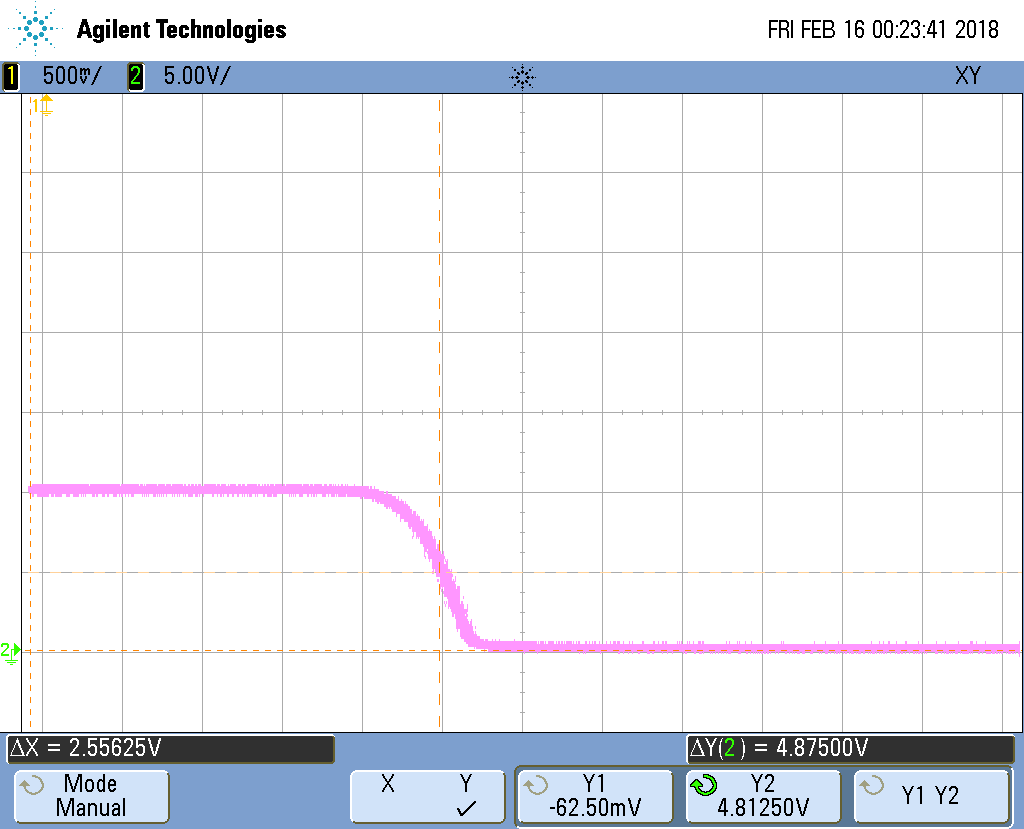
\includegraphics[scale=0.75]{../img/scope_0}
	\caption{The output of our oscilloscope for the voltage transfer curve of the circuit shown in figure \ref{fig:vtc_circuit}.}
	\label{fig:vtc_result}
\end{figure}
\FloatBarrier

